\tikzset{
  compass/.pic = {
    \foreach[count=\i,evaluate={\m=mod(\i-1,2);\a=90*\i;\n=-(180*\m+\a)}]
    \d in {N,W,S,E} {
      \filldraw[fill=lightgray, pic actions,rotate=\a] (0,0) -- (45:0.35)--(0:1)
          node[auto=right,anchor=\n,transform shape,rotate=-\a]{\d};
      \filldraw[pic actions,fill=white,rotate=\a]
          (0,0) -- (-45:0.35)--(0:1)--cycle;
    };
  }
}



\newcommand*{\TODO}[1]{\textsf{TODO: #1}}

Denne opgave går ud på at implementere en variant af brætspillet
\emph{Ricochet Robots} (først udgivet i tyskland under navnet
\emph{Rasende Roboter}
\url{http://en.wikipedia.org/wiki/Ricochet_Robot}).

I denne opgave skal der arbejdes med at lave et objekt-orienteret
design, som gør det nemt at udvide spillet med nye regler og elementer.

\TODO{Skriv opsummering} Opgaven er delt i fire dele. I den første delopgave skal der arbejdes
med at implementere en \emph{canvas} i terminalen til at vise vores
verden. Anden delopgave går ud på at lave et klasse-hierarki til at
repræsentere skabninger og genstande i verden. Endelig skal der i den
tredie delopgave arbejdes mod at sætte de forskellige dele sammen til
et samlet spil. Fjerde del indeholde en række forslag til udvidelser,
hvoraf I skal implementere mindst to.

I det følgende er der kun givet minimums-krav til hvilke metoder og
properties I skal implementere på jeres klasser. I må gerne lave
ekstra metoder eller hjælpe-funktioner, hvis I synes det kan hjælpe
jer med at skrive et mere elegant og forståeligt program.

%\textbf{Rapport}

\subsection*{Rapport}


Ud over jeres programkode skal I også aflevere en rapport (skrevet i
\LaTeX). I rapporten skal I beskrive implementeringen af jeres
klasser, det vil sige hvilken skjult tilstand (interne variable og
lignende), som jeres metoder arbejder på.

Ligeledes skal rapporten indeholde et UML diagram over klasserne i
jeres løsning.

\subsection*{Spillets basisregler}
\label{sec:spillets-basisregler}

Spillet foregår på en \emph{plade} med $r \times c$ felter, det vil
sige $r$ rækker og $c$ kolonner, hvor et antal
\emph{robotter} kan flyttes rundt. Hver robot starter i et separat felt på
pladen, og kan derefter flyttes ved at \emph{glide} i en af de fire
retninger \emph{nord}, \emph{syd}, \emph{øst} eller \emph{vest}. Målet
med spillet er at få flyttet en af robotterne hen til et
\emph{målfelt} i det laveste antal træk. Udfordringen er at når en
robot starter med at glide i en retning så fortsætter den med at glide
i den retning indtil, at den rammer enten en væg eller en anden
robot. For at gennemføre et spil, skal en robot stoppe i et
målfelt. Det tæller ikke som en løsning, hvis en robot blot glider
gennem målfeltet.

\begin{figure}
  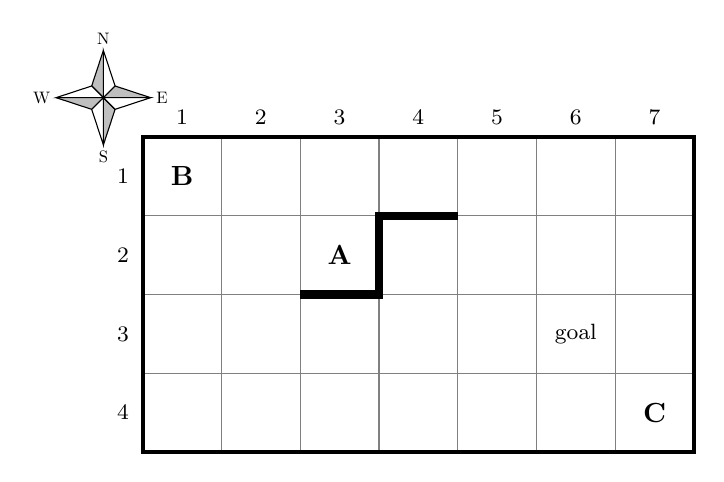
\begin{tikzpicture}[baseline=0]
  \pic[scale=.6] at (-0.5,0.5) {compass};
  \draw[step=10mm,color=gray,thin] (0,0) grid (7,-4);
  \draw[ultra thick] (0,0) rectangle (7,-4);
  \foreach \col in {1,...,7} {
    \node at (\col-0.5, 0.25) {\footnotesize\col};
  };
  \foreach \row in {1,...,4} {
    \node at (-0.25, 0.5-\row) {\footnotesize\row};
  };

  \draw[line width=3pt] (2,-2) -- (3,-2) -- (3,-1) -- (4,-1);
  \begin{scope}[shift={(-0.5,0.5)}]
  \node at (1,-1) {\textbf{B}};
  \node at (3,-2) {\textbf{A}};
  \node at (7,-4) {\textbf{C}};
  \node at (6,-3) {\footnotesize{}goal};
  \end{scope}
\end{tikzpicture}
\hfill
\begin{minipage}[t]{0.4\linewidth}
  \raggedright\setlength{\parskip}{1ex}
  Spilleplade med $4\times 7$ felter.

  Robotter: \textbf{A} i felt~(2,3), \textbf{B} i felt~(1,1) og
  \textbf{C} i felt~(3,6).

  Indre vægge, tre stk: vertikal, 1~felt, øst,
startfelt~(2,3); horisontal, 1~felt, syd, startfelt~(2,3); horisontal,
1~felt, syd, startfelt~(1,4).

  Målfelt: (3,6) $(3,6)$
\end{minipage}
  \caption{Eksempel startposition}
  \label{fig:example}
\end{figure}

Figur~\ref{fig:example} viser et eksempel på en startposition for et
spil. Dette spil kan fx løses i seks træk: flyt \textbf{A} nord, flyt
\textbf{A} øst, flyt \textbf{A} syd, flyt \textbf{C} vest, flyt
\textbf{B} syd, flyt \textbf{B} øst. Der er 24 forskellige løsninger
på 6 træk til spillet i Figur~\ref{fig:example}, og ingen der er
kortere end 6~træk.

%%% Local Variables:
%%% mode: latex
%%% TeX-master: "main"
%%% End:
